\subsection{Mốc so sánh}
Trên bốn bộ dữ liệu này, công trình cùng bài toán, cùng đầu vào và có công bố sai số theo từng nhóm cell kiểm tra là PINN4SOH~\cite{wang2024}. Bài đó còn báo cáo hai mô hình đối chứng MLP và CNN trên cùng các nhóm. Các bài công bố bộ dữ liệu gốc giải bài toán khác hoặc dùng đầu vào khác: Severson và cộng sự~\cite{severson2019} dự đoán tuổi thọ của cả cell từ các chu kỳ đầu, Zhu và cộng sự~\cite{zhu2022} dùng điện áp hồi phục sau sạc, Ma và cộng sự~\cite{ma2022} dùng học chuyển giao với cách chia riêng. Vì cách chia và đầu vào khác nhau, sai số của các bài đó không so trực tiếp được với đồ án, và báo cáo không trích chúng. Mọi so sánh dưới đây dùng đúng 39 nhóm đánh giá của bài, dựng lại từ nhật ký huấn luyện công bố kèm mã: mỗi nhóm thí nghiệm (batch) của XJTU và TJU là một nhóm đánh giá ở chế độ đầy đủ, một nhóm cho MIT (23 cell kiểm tra) và cho HUST (20 cell kiểm tra), và các nhóm ít mẫu $K = 1, \dots, 4$ của XJTU và HUST. Sai số tính đúng như bài: MAE từng cell kiểm tra, trung bình qua lần chạy, qua cell, qua nhóm. PINN-lai của đồ án chạy với hai cách tiền xử lý: bản sao tiền xử lý của bài (có rò rỉ, chỉ để so cùng điều kiện) và tiền xử lý không rò rỉ của đồ án. Bảng~\ref{tab:pub} và \Cref{fig:bench} tập hợp các con số.

\begin{table}[!htbp]\centering\small\setlength{\tabcolsep}{5pt}
\caption[So với PINN4SOH trên đúng cách chia của bài]{MAE theo cell ($\times10^{-3}$) trên đúng 39 nhóm đánh giá của bài PINN4SOH, trung bình qua cell kiểm tra, lần chạy và nhóm như bài; $K$ là số cell có nhãn trong thí nghiệm ít mẫu. Ba cột đầu là số công bố của bài cho PINN4SOH và hai mô hình đối chứng MLP, CNN của bài. Cột chạy lại: mã gốc của bài chạy trên đúng các nhóm đó, siêu tham số theo nhật ký của bài, 10 lần mỗi nhóm. Hai cột cuối: PINN-lai của đồ án (3 hạt giống) với tiền xử lý của bài, cùng điều kiện với các cột trước, và với tiền xử lý không rò rỉ. In đậm: thấp nhất trong năm cột cùng điều kiện. $^{*}$/$^{\dagger}$: PINN-lai với tiền xử lý của bài thấp hơn/cao hơn có ý nghĩa thống kê so với mã gốc chạy lại (Wilcoxon ghép cặp theo cell kiểm tra, Holm qua 12 hàng).}\label{tab:pub}
\begin{adjustbox}{max width=\textwidth}\begin{tabular}{llrrrrrr}\toprule
 & & \multicolumn{6}{c}{MAE theo cell ($\times10^{-3}$) $\downarrow$} \\\cmidrule(lr){3-8}
 & & \multicolumn{3}{c}{số công bố của bài} & PINN4SOH & \multicolumn{2}{c}{PINN-lai của đồ án} \\\cmidrule(lr){3-5}\cmidrule(lr){6-6}\cmidrule(lr){7-8}
Bộ & Chế độ & PINN4SOH & MLP & CNN & chạy lại & tiền xử lý của bài & không rò rỉ \\\midrule
XJTU & đầy đủ & 7{,}85 & 21{,}02 & 21{,}19 & 8{,}66 & \textbf{6{,}62} & 7{,}81 \\
TJU & đầy đủ & 9{,}79 & 13{,}61 & 12{,}66 & 11{,}21 & \textbf{8{,}78}$^{*}$ & 6{,}16 \\
MIT & đầy đủ & 6{,}18 & 7{,}45 & \textbf{6{,}15} & 7{,}36 & 6{,}80 & 1{,}43 \\
HUST & đầy đủ & 7{,}57 & 7{,}77 & 7{,}21 & 7{,}90 & \textbf{6{,}45}$^{*}$ & 12{,}51 \\
\addlinespace
XJTU & $K = 1$ & 31{,}54 & 49{,}14 & 131{,}16 & 30{,}70 & \textbf{10{,}51}$^{*}$ & 13{,}27 \\
 & $K = 2$ & 10{,}06 & 24{,}88 & 62{,}80 & 11{,}54 & \textbf{7{,}72} & 13{,}60 \\
 & $K = 3$ & 7{,}98 & 23{,}59 & 49{,}96 & 9{,}24 & \textbf{7{,}15} & 9{,}48 \\
 & $K = 4$ & 7{,}62 & 22{,}60 & 38{,}62 & 9{,}17 & \textbf{7{,}20} & 8{,}39 \\
\addlinespace
HUST & $K = 1$ & 39{,}42 & 50{,}37 & 112{,}78 & 47{,}13 & \textbf{14{,}71}$^{*}$ & 46{,}72 \\
 & $K = 2$ & 16{,}94 & 36{,}00 & 65{,}04 & 18{,}07 & \textbf{11{,}53}$^{*}$ & 23{,}82 \\
 & $K = 3$ & 14{,}59 & 22{,}99 & 43{,}71 & 15{,}10 & \textbf{9{,}16}$^{*}$ & 21{,}13 \\
 & $K = 4$ & 13{,}62 & 24{,}04 & 36{,}74 & 14{,}71 & \textbf{9{,}91}$^{*}$ & 22{,}64 \\
\bottomrule\end{tabular}\end{adjustbox}\end{table}

\begin{figure}[!htbp]\centering
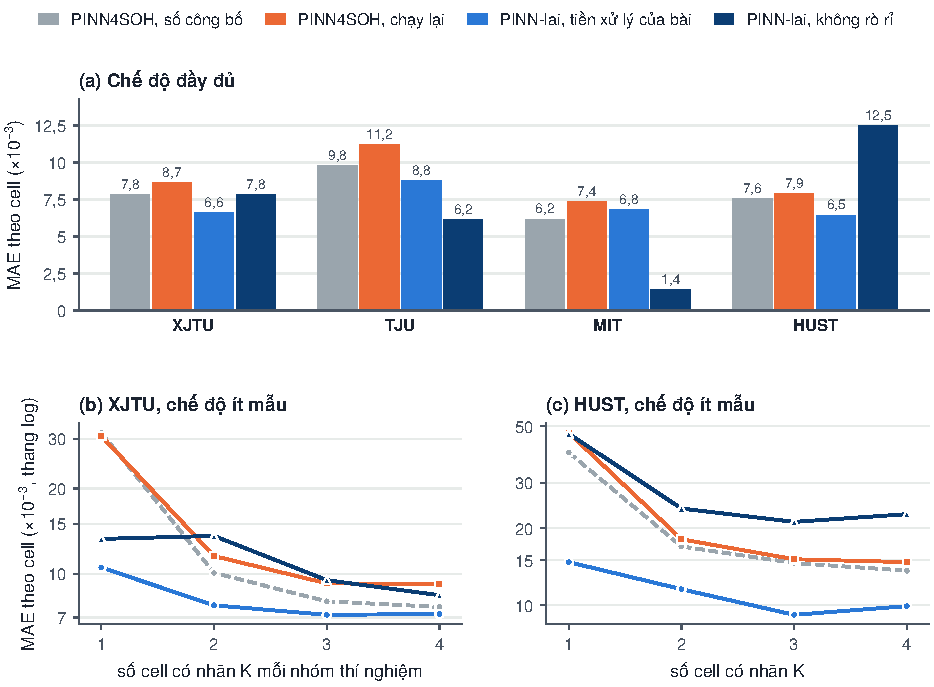
\includegraphics[width=\textwidth]{graphics/fig_benchmark.pdf}
\caption[So với PINN4SOH trên đúng cách chia của bài]{MAE theo cell trên đúng các nhóm đánh giá của bài PINN4SOH. (a) Chế độ đầy đủ, mỗi bộ bốn cột: số công bố của bài, mã gốc của bài chạy lại, PINN-lai với tiền xử lý của bài và PINN-lai với tiền xử lý không rò rỉ. (b), (c) Chế độ ít mẫu: MAE theo số cell có nhãn $K$.}\label{fig:bench}
\end{figure}

Theo RMSE, Bảng~\ref{tab:pubrmse} lấy trên mỗi bộ mô hình có sai số thấp nhất của đồ án và ghi tên mô hình đó. RMSE thấp nhất của đồ án thấp hơn số công bố ở XJTU, TJU và HUST (XJTU: PINN-lai, 22{,}2\,\%; TJU: PINN-lai, 14{,}0\,\%; HUST: PINN-lai, 16{,}3\,\%). Ở MIT, GBDT cao hơn 0{,}2\,\%.

\begin{table}[!htbp]\centering\small
\caption[RMSE tốt nhất của đồ án so với PINN4SOH]{RMSE ($\times10^{-3}$) trên đúng cách chia của bài PINN4SOH, chế độ đầy đủ, cùng tiền xử lý với bài. Cột thứ hai tính từ tệp kết quả công bố cùng mã nguồn của bài; cột thứ ba là RMSE thấp nhất trong PINN-lai, GBDT và PINN-semi của đồ án, cột Mô hình ghi mô hình đạt được. Cả hai cột lấy trung bình qua cell kiểm tra, lần chạy và nhóm như Bảng~\ref{tab:pub}. In đậm: thấp hơn trong hai cột. Chênh lệch là RMSE của đồ án so với số công bố, âm là đồ án thấp hơn.}\label{tab:pubrmse}
\begin{tabular}{lrrlr}\toprule
Bộ dữ liệu & RMSE PINN4SOH công bố $\downarrow$ & RMSE tốt nhất của đồ án $\downarrow$ & Mô hình & Chênh lệch $\downarrow$ \\\midrule
XJTU & 10{,}88 & \textbf{8{,}47} & PINN-lai & $-$22{,}2\,\% \\
TJU & 12{,}28 & \textbf{10{,}56} & PINN-lai & $-$14{,}0\,\% \\
MIT & \textbf{7{,}51} & 7{,}52 & GBDT & $+$0{,}2\,\% \\
HUST & 8{,}69 & \textbf{7{,}27} & PINN-lai & $-$16{,}3\,\% \\
\bottomrule\end{tabular}\end{table}

\subsection{Các chỉ số tốt hơn các bài báo đã công bố}
Cùng cách chia và cùng tiền xử lý với bài, PINN-lai có sai số thấp hơn mã gốc PINN4SOH chạy lại ở 12 trên 12 chế độ, thấp hơn có ý nghĩa thống kê ở 7 (tỉ số 0{,}76--0{,}92 ở chế độ đầy đủ, 0{,}31--0{,}79 ở chế độ ít mẫu) và không chế độ nào cao hơn có ý nghĩa thống kê (Bảng~\ref{tab:pub}). So với số công bố của PINN4SOH, PINN-lai thấp hơn ở 11 trên 12 chế độ (tỉ số 0{,}84--1{,}10 ở chế độ đầy đủ, 0{,}33--0{,}94 ở chế độ ít mẫu). Lợi thế lớn nhất ở chế độ ít mẫu, nơi hàm mất mát vật lý được tính cả trên các cell huấn luyện không nhãn. So với MLP và CNN mà bài PINN4SOH báo cáo, PINN-lai thấp hơn MLP ở 12 trên 12 chế độ và thấp hơn CNN ở 11 trên 12. Với tiền xử lý không rò rỉ, PINN-lai vẫn thấp hơn số công bố của PINN4SOH trên TJU (tỉ số 0{,}63), MIT (tỉ số 0{,}23), thấp hơn có ý nghĩa thống kê theo cell ở 2 trên 4 bộ đầy đủ, và ở XJTU $K = 1$ (tỉ số 0{,}42).

\subsection{Các chỉ số chưa tốt}
So với các bài báo đã công bố, đồ án còn một số điểm chưa đạt. Cùng điều kiện với bài, PINN-lai chưa thấp hơn số công bố của PINN4SOH ở MIT đầy đủ (6{,}80 so với 6{,}18), và chưa thấp hơn CNN của bài ở MIT đầy đủ (6{,}15). Một GBDT đơn giản với cùng tiền xử lý rò rỉ tốt ngang PINN-lai: tỉ số GBDT/PINN-lai 0{,}69--1{,}06, GBDT thấp hơn có ý nghĩa thống kê ở 2 chế độ (HUST $K = 1$, HUST $K = 2$) và không chế độ nào cao hơn. Với min--max theo cell, chỉ số chu kỳ đã chuẩn hoá là phần đời đã qua và mô hình cây khai thác thẳng thông tin này, nên lợi thế so với mã gốc trong điều kiện đó không thể quy cho phần vật lý. Với tiền xử lý không rò rỉ, PINN-lai cao hơn số công bố trên HUST (tỉ số 1{,}65), ngang trên XJTU (0{,}99), cao hơn có ý nghĩa thống kê theo cell ở 1 trên 4 bộ đầy đủ. Ở chế độ ít mẫu cao hơn ở 7 trên 8 (tỉ số 1{,}10--1{,}66). Đây là các chế độ mà tiền xử lý của bài có lợi nhiều nhất: khi chỉ có vài cell có nhãn, biết cell đã đi được bao nhiêu phần đời gần như là biết SOH. Đồ án không dùng tiền xử lý đó vì nó không thực hiện được khi triển khai (Mục~\ref{sec:dt_bo}). Đồ án không tái lập được chính xác số công bố của PINN4SOH: mã gốc chạy lại cho sai số bằng 1{,}04--1{,}19 lần ở chế độ đầy đủ, cao hơn có ý nghĩa thống kê theo cell ở 2 trên 4 bộ (Bảng~\ref{tab:pub}). Các hàng huấn luyện dựng lại trùng với dữ liệu của bài, nên phần chênh đến từ phần cứng và phiên bản thư viện.

Ngay trong các so sánh của chính đồ án, một số chỉ số cũng chưa đạt. GBDT đơn lẻ có sai số thấp hơn PINN-semi ở 14/16 trường hợp bộ $\times$ mức nhãn (10 có ý nghĩa thống kê). PINN-semi chỉ vượt GBDT có ý nghĩa thống kê ở HUST 30\,\% nhãn (Mục~\ref{sec:labels}). PINN-lai cố định vẫn kém GBDT có ý nghĩa thống kê ở TJU 70\,\%. Ở 70\,\% nhãn, PINN-semi kém MLP có ý nghĩa thống kê trên TJU (tỉ số 1{,}09). Với kiểm định bảo thủ ở mức fold, lợi ích ở 30\,\% nhãn chỉ đứng vững trên MIT. Khoảng dự đoán 90\,\% của ước lượng SOH có độ phủ thực tế 84{,}9--92{,}6\,\% (trung bình 88{,}8\,\%), 14--25\,\% số cell có độ phủ dưới 80\,\%. Với HiPINN (\Cref{sec:e33res}), khoảng SOH 90\,\% tính bằng phương pháp conformal phủ 89--93\,\% tuỳ bộ và ngân sách, khoảng RUL 90\,\% phủ 68--87\,\%. Tỉ lệ dự báo RUL nằm trong $\pm 20\,\%$ RUL thật là 53--84\,\%. Ở 10\,\% đời cuối của XJTU, MAE của HiPINN vẫn là 30{,}0 ($\times10^{-3}$). Tham số vật lý $\lambda$, $E_a$ không được dữ liệu xác định, và tốc độ $r$ học được thấp hơn nhiều tốc độ suy giảm thực đo (\Cref{sec:vatly}). Bộ lọc xu thế không bảo đảm SOH dự đoán không tăng (đầu ra tăng ở 28--44\,\% số bước). Ép không tăng làm sai số trên XJTU tăng 1{,}76--1{,}94 lần vì dung lượng đo được của XJTU tăng ở đầu đời.

\subsection{Vai trò của phần vật lý}\label{sec:vatly}
Đề tài nhấn mạnh sự hỗ trợ của thông tin hoá lý, nên cần nói rõ phần vật lý trong PINN-semi thực sự đóng góp gì. Ba quan sát ở các mục trước cho thấy đóng góp này hẹp hơn tên gọi. Thứ nhất, chỉ riêng ràng buộc đơn điệu đã mang lại 62--95\,\% mức giảm sai số của PINN-semi so với MLP ở 30\,\% nhãn, còn bỏ phần dư động học và ràng buộc miền chỉ làm MAE tăng 1--11\,\% (\Cref{sec:source}). Thứ hai, các tham số hoá lý dịch chuyển ít so với giá trị khởi tạo: $\lambda$ (khởi tạo bằng 1) của các PINN-semi nằm trong khoảng 0{,}96--0{,}98 ở XJTU, 0{,}95--0{,}97 ở TJU, 0{,}95--0{,}97 ở MIT và 0{,}90--1{,}26 ở HUST, còn $E_a$ khởi tạo ở 30\,kJ/mol thì dịch không quá 1{,}6\,kJ/mol. Thứ ba, tốc độ $r$ học được trung bình chỉ 0{,}001--0{,}063, trong khi tốc độ suy giảm thực đo là 0{,}137--0{,}356 SOH trên 1\,000 chu kỳ. Cả ba có nguyên nhân trong cách đặt bài toán, không phải do tối ưu chưa hội tụ.

Phần dư động học ràng buộc đạo hàm riêng $\partial u/\partial t$ khi giữ nguyên đặc trưng sạc. Trên quỹ đạo thật của một cell, SOH thay đổi chủ yếu vì đặc trưng sạc thay đổi theo tuổi, tức qua số hạng $\nabla_{\mathbf{x}} u \cdot \mathrm{d}\mathbf{x}/\mathrm{d}n$, còn $t$ chỉ là một trong 17 đầu vào. Mạng nghiệm vì vậy thoả được phương trình với một đạo hàm riêng nhỏ theo $t$, và $r$ học được nhỏ hơn nhiều so với tốc độ suy giảm thật. Với trọng số $\alpha = 0{,}02$, phần dư này chủ yếu buộc đạo hàm theo $t$ không dương, điều mà ràng buộc đơn điệu đã làm trực tiếp hơn.

Hệ số $\lambda$ khó xác định vì thừa số $g(u) = e^{\lambda(1-u)}$ chỉ thay đổi khoảng 22\,\% khi SOH đi từ 1 xuống 0,8 với $\lambda \approx 1$. Sự phụ thuộc vào mức suy giảm này đã có sẵn trong $k(\tilde{\mathbf{x}})$, vốn nhận các đặc trưng sạc biến thiên theo tuổi. Hai thừa số thay thế được cho nhau, nên dữ liệu chỉ kéo $\lambda$ đi một đoạn ngắn khỏi giá trị khởi tạo, xa nhất ở HUST.

Năng lượng hoạt hoá $E_a$ thì không định danh được về mặt toán học trên ba bộ. Thừa số Arrhenius $A(T) = \exp[-(E_a/R_g)(1/T - 1/T_\text{ref})]$ chỉ khác 1 khi nhiệt độ khác $T_\text{ref}$. Ở XJTU, mọi cell chạy ở 298{,}15\,K, đúng bằng $T_\text{ref}$, nên $1/T - 1/T_\text{ref} = 0$, $A \equiv 1$ và gradient của hàm mất mát theo $E_a$ bằng 0. Thực tế $E_a$ của mọi PINN-semi trên XJTU giữ đúng 30{,}0\,kJ/mol. Ở MIT và HUST, nhiệt độ là hằng 303{,}15\,K, nên $A$ chỉ là một hằng số nhân và bị $k(\tilde{\mathbf{x}}) = \operatorname{softplus}(G_\theta(\tilde{\mathbf{x}}))$ hấp thụ: mọi giá trị $E_a$ cho cùng một $r$ nếu $G_\theta$ bù lại. Chỉ TJU có ba mức nhiệt độ (298{,}15, 308{,}15 và 318{,}15\,K), nơi $E_a$ về nguyên tắc định danh được. Nhưng ở đó nhiệt độ chỉ làm sai số thay đổi dưới 1\,\% (thêm $1/T$ vào GBDT cho tỉ số 0{,}99--1{,}00, \Cref{sec:dt_bo}), nên dữ liệu cũng không đủ để ước lượng $E_a$ chính xác.

Dù vậy, phần vật lý vẫn có giá trị ở ba điểm. Một là ràng buộc đơn điệu và ràng buộc miền là tiên nghiệm vật lý đúng, và chúng được áp lên cả cell không nhãn. Ở 10\,\% nhãn, phần lợi ích do áp hàm mất mát vật lý lên cell không nhãn (PINN-semi so với PINN-sup, tỉ số 0{,}62--0{,}94) chiếm 50--64\,\% mức giảm sai số so với MLP. Hai là dạng tốc độ có cấu trúc, luôn không âm, ngăn lời giải tầm thường $G \approx u_t$ của động học hộp đen kiểu PINN4SOH, nên các ràng buộc thực sự tác động lên mạng nghiệm. Ba là ở bài toán dự báo, nghiệm đóng của cùng động học xám cho PINN-dự báo một đường ngoại suy có dạng vật lý: luôn không tăng, có thể gãy dần hoặc chậm dần, với chỉ hai tham số. PINN-dự báo là một trong ba nhánh của HiPINN. Vì vậy cụm “thông tin hoá lý” trong đồ án nên được hiểu là các tiên nghiệm có cấu trúc (đơn điệu, miền giá trị, tốc độ không âm, dạng Arrhenius, dạng nghiệm đóng), chứ không phải việc xác định các tham số điện hoá của cell.

\subsection{Nhận xét}
Trên đúng cách chia của PINN4SOH và cùng cách tính sai số, PINN-lai của đồ án có sai số thấp hơn số công bố ở phần lớn các chế độ và thấp hơn mã gốc chạy lại ở mọi chế độ. Tuy vậy, trong điều kiện có rò rỉ của bài, một GBDT cũng đạt kết quả tương tự, còn khi bỏ rò rỉ thì hơn hay kém tuỳ bộ dữ liệu. Vì thế, những đóng góp có cơ sở vững nhất của đồ án là giao thức đánh giá không rò rỉ, các so sánh ghép cặp có kiểm định trong cùng một giao thức, và các mô hình có đặc trưng lịch sử HiGBDT, HiPINN cho bài toán dự báo.
